\let\negmedspace\undefined
\let\negthickspace\undefined
\documentclass[journal]{IEEEtran}
\usepackage[a5paper, margin=10mm, onecolumn]{geometry}
%\usepackage{lmodern} % Ensure lmodern is loaded for pdflatex
\usepackage{tfrupee} % Include tfrupee package

\setlength{\headheight}{1cm} % Set the height of the header box
\setlength{\headsep}{0mm}     % Set the distance between the header box and the top of the text

\usepackage{gvv-book}
\usepackage{gvv}
\usepackage{cite}
\usepackage{amsmath,amssymb,amsfonts,amsthm}
\usepackage{algorithmic}
\usepackage{graphicx}
\usepackage{textcomp}
\usepackage{xcolor}
\usepackage{txfonts}
\usepackage{listings}
\usepackage{enumitem}
\usepackage{mathtools}
\usepackage{gensymb}
\usepackage{comment}
\usepackage[breaklinks=true]{hyperref}
\usepackage{tkz-euclide} 
\usepackage{listings}
% \usepackage{gvv}                                        
\def\inputGnumericTable{}                                 
\usepackage[latin1]{inputenc}                                
\usepackage{color}                                            
\usepackage{array}                                            
\usepackage{longtable}                                       
\usepackage{calc}                                             
\usepackage{multirow}                                         
\usepackage{hhline}                                           
\usepackage{ifthen}                                           
\usepackage{lscape}
\begin{document}

\bibliographystyle{IEEEtran}
\vspace{3cm}

\title{
1-Vector Arithmetic \\
\large EE1030:Matrix Theory
}
\author{Gajjarapu Satyanarayana\\AI24BTECH11009
}
% \maketitle
% \newpage
% \bigskip
{\let\newpage\relax\maketitle}

\renewcommand{\thefigure}{\theenumi}
\renewcommand{\thetable}{\theenumi}



\numberwithin{equation}{enumi}
\numberwithin{figure}{enumi}
\renewcommand{\thetable}{\theenumi}


\textbf{Question}:1.7.6\\
Find a relation between $x$ and $y$ if the points \textbf{A}($x,y$), \textbf{B}(-4,6), and  \textbf{C}(-2,3)\hfill(10, 2019)\\ are collinear.
\\
\textbf{Solution:}
\renewcommand{\tablename}{Table 1.7.6.1}
\begin{table}[h!]
  \centering
  \begin{tabular}[12pt]{ |c| c|}
    \hline
    \textbf{Variables} & \textbf{Description}\\ 
    \hline
    $\textbf{V}_1, \vec{u}_1, f_1$ & Parameters of the parabola $y^2 = 4x$ \\
    \hline
     $\textbf{V}_2, \vec{u}_2, f_2$ & Parameters of the circle $4x^2 + 4xy^2 = 9$ \\
    \hline
    $\vec{x}^\intercal\brak{\textbf{V}_1 + \mu\textbf{V}_2}\vec{x} + 2\brak{\vec{u}_1 + \mu\vec{u}_2}^\intercal\vec{x} + \brak{f_1 + \mu f_2}$ & Intersection of two conics \\
    \hline
    \end{tabular}


  \caption{Vertex and its coordinates}
\end{table}
\\
 Points \textbf{A}, \textbf{B}, \textbf{C} are said to be collinear if
 \begin{align}
	 & rank\myvec{\vec{B} - \vec{A} & \vec{C} - \vec{A}} = 1 \label{eq1.7.6.1} \\ &
	 \vec{B} - \vec{A} = \myvec{-4 \\ 6} - \myvec{x \\ y} \\ &
	 \vec{B} - \vec{A} = \myvec{-4 - x \\ 6 - y} \\ &
	 \vec{C} - \vec{A} = \myvec{-2 \\ 3} - \myvec{x \\ y} \\ &
	 \vec{C} - \vec{A} = \myvec{-2 - x \\ 3 - y} \\ &
	 \myvec{\vec{B} - \vec{A} & \vec{C} - \vec{A}} = \myvec{-4 - x & -2 - x \\ 6 - y & 3 - y} \\ &
	 \myvec{-4 - x & -2 - x \\ -6 - y & 3 - y} \xrightarrow[]{R_2 \rightarrow R_1+\frac{2}{3}R_2} \myvec{-4 - x & -2 - x \\ -x - \frac{2}{3}y & -x - \frac{2}{3}y} \\ &
     \end{align}
Given \textbf{A}, \textbf{B}, \textbf{C} are collinear, so rank\myvec{\vec{B} - \vec{A} & \vec{C} - \vec{A}} = 1 from equation \ref{eq1.7.6.1} \\
Therefore,
\begin{align}
	& -x - \frac{2}{3}y = 0 \\ &
	x = - \frac{2}{3}y \\ &
	3x = -2y \\ &
	3x + 2y = 0 \\ &
\end{align}
The relation between $x$ and $y$ is $3x + 2y = 0$.
\begin{figure}[h!]
   \centering
   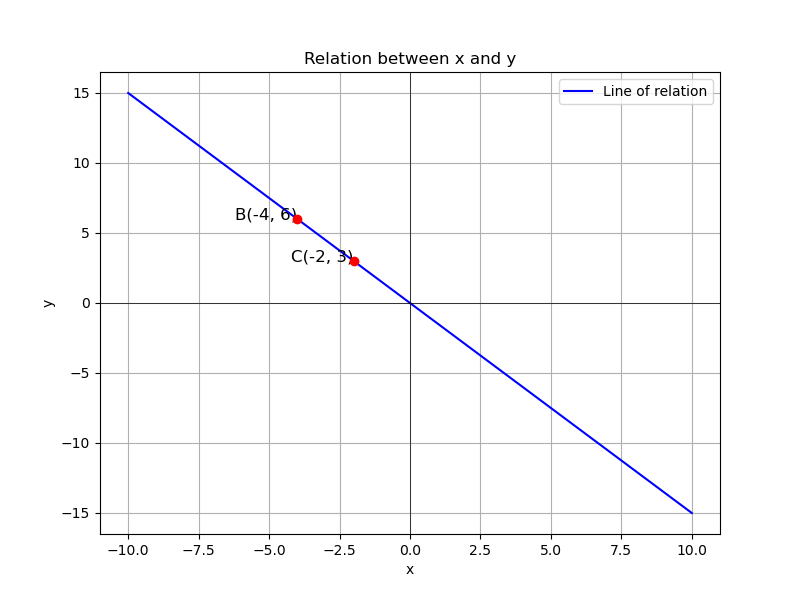
\includegraphics[width=0.7\linewidth]{figs/collinear.png}
   \caption{Relation between $x$ and $y$: $3x + 2y = 0$}
   \end{figure}
   \end{document}
